
\chapter{Introduction}

In the modern world, data is increasingly important for decision making. While
one side of this development is the world of big data, where more and more data
enters bigger and bigger models, another side is the world of small data sets
with non-stationary distributions. Electricity demand forecasts, TODO, TODO
all of these involve forecasting based on small amounts of data, where we know
that the data distribution changes over time. TODO

% In low-data environments, attaining more data can be useful. Often, though,
% relevant data is owned by a competitor, and parties will not be willing to give
% data to each other. Otherwise, data could come from a party that needs to 

%However, in these situations,
% actors in competition often end up with data that would be valuable for several
% parties, but with no incentive to share data between them.

% In the decades TODO and TODO, two developments started to happen side by side.
% Computers started enabling autonomous collection and organization of data,
% which gave us for the first time access to larger datasets about the real
% world. At the same time, computers also allowed us to use that data through
% both increased computational power and the development of more advanced methods
% of presenting and displaying said data for an end user. TODO:REF. Business
% intelligence as a term appeared in the year TODO, and the relational database
% was first introduced in the 1970 paper TODO:REF. These innovations and others
% started allowing organizations to structure and interrogate their data faster
% and more easily.

\section{Data Sharing}

Since decisions first started to be made based on data, people started to
realize the gains they could get from using other people's data. This inspired
early research into what is known as data sharing TODO:REF where multiple
parties freely share their data with each other so that all parties can gain
from it.

Data sharing was first studied in the context of sharing with no external
incentive, e.g. within the research on federated learning. Federated learning
is an approach for training machine learning models in a decentralized manner
where other people's data can be used while preserving their private knowledge
of their own data, thus letting people share data without any cost for the loss
of privacy. TODO:REF Even though this removes negative effects from loss of
privacy to the data owners, this is still not enough to incentivize data
sharing for two central reasons:

\begin{enumerate}
  \item There is some cost associated with preparing and providing data for
    sharing, which a participant would have to bear altruistically without any
    return.
  \item Participants might be competitors in a downstream market. In
    the dayahead electricity market, for example, improving the prediction of a
    competitor could potentially leave you worse off as they outperformed you
    in the market.
\end{enumerate}


\section{Emergence of Data Markets}
To incentivize sharing for data owners, data markets were developed where
participants receive compensation for providing their data. Initial data
markets were developed as a way to monetize data samples, or what would in
tabular data be known as a row of data. TODO:REF This kind of information
covers e.g. the information that a social network site has about its customers
- the site knows about a number of people and sells off the information that it
has about a single person as a bundle. Examples of this kind of marketplace are
the Snowflake or AWS data exchanges.

Another kind of data marketplace is the prediction marketplace. This kind of
market does not sell data for use in one's own predictions, but instead directly
sells predictions. These are generally set up basically like a gambling site,
where parties bet on an outcome of a real-world event and get paid based on
whether they bet correctly. While prediction markets often basically boil down
to political gambling sites, other styles of prediction markets do exist, e.g.
predicting the prices of bonds or futures. In a certain way, the entire futures
market can be seen as a prediction marketplace as people predict future prices
of wares. TODO:REF

\section{Motivation for Analytics Markets}

Let us now turn to a different situation where data from others can be useful.
Let us imagine first a single renewable generating participant in the
electricity market, say that it is a wind farm. The electricity market
generally works by participants selling electricity a day before it is
used in a market known as the dayahead electricity market. The electricity is then
consumed at what is known as imbalance time. Renewable generation depends on
weather circumstances, meaning that the actual generation at imbalance time can
only be forecasted when selling in the dayahead market.

The system is run by the \emph{balancing party}, which is in charge of ensuring
that the real-time power demand will be met by producers. The balancing party
wants the best possible prediction of the real-time power generation at
dayahead time, as incorrect forecasts might lead to over- or under production
of electricity at real time, which the balancing party must then fix by paying
for reserve resources to either start up or shut down. TODO:REF

This wind farm must decide how much power to sell in the dayahead electricity
market. It wants to be as close as possible to its true generation at imbalance
time. If it overestimates its production and sells too much power, it will have
to pay the imbalance price to make up for the power it is unable to produce. If
it instead underestimates its production and sells too little power, it will
not be making money from the extra generation it could have sold. Its profit is
then a function of its prediction accuracy. The single wind farm is illustrated
in figure \ref{fig:single_wind_farm}, where we see its bid as a function of its
production forecast.

\begin{figure}
  \centering
  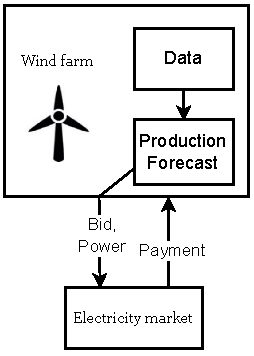
\includegraphics[width=2in]{Pictures/single_wind_farm.pdf}
  \caption{A single wind farm in the electricity market, using its own data to
  forecast its production at imbalance time, and supplying bids based on this.
  The payment is then based on the produced power and the dayahead electricity
  price. However, if the farm undershoots its production, it will have surplus
  energy at imbalance time that it needs to get rid of, and if it overshoots
  its production, it must itself pay the imbalance price for the missing energy
  to make it up. TODO: OKAY DESCRIPTION?}
  \label{fig:single_wind_farm}
\end{figure}

This wind farm makes a multi time horizon prediction based on some data that it
has available. Maybe it has some sensors, some current production data, etc.
Now, let us say that the wind farm has another competitor in the market -
another wind farm. We then have two participants in the market who both will
earn more the better their prediction is.

Intuitively, data from competing wind farms will improve forecasting accuracy.
This was also shown in TODO: REF TASTU 2013. Both farms would be able to
better predict their production if they had access to each other's data. This
would not only benefit the two wind farms, but also the balancing party, as
they would have a better incoming prediction of total available generation and
thus the total cost of balancing would be lower. TODO: REF This means that the
societal social welfare would be increased if the participants shared data.
They might not be willing to share data, however, since they are in direct
competition in the dayahead energy market, so one wind farm might be more
penalized by the improvement in the prediction capability of the other wind
farm than they are rewarded by their increase in predictive power.

To facilitate this data exchange, we can introduce a new type of data market,
known as an analytics market. The word analytics market refers to many things
in literature but in this thesis it refers to a specific kind of data
marketplace, also known as a regression market or classification market. Where
the previously discussed markets traded either data samples or predictions,
sellers in analytics markets instead sell features, or what in tabular datasets
are known as columns. Some machine learning method then transforms the features
into predictions, and these are bought by the buyers. The market structure can
be seen in figure \ref{fig:analytics_market}. Since this requires features to
pertain to the same observation or row, the market is often based on time
series problems, where sellers provide features for a single time point and
buyers buy predictions for that time point. This is the structure of the
problem in our motivating example. A single time step of the analytics market
is shown in figure \ref{fig:analytics_market_time_step}. TODO:REF

\begin{figure}
  \centering
  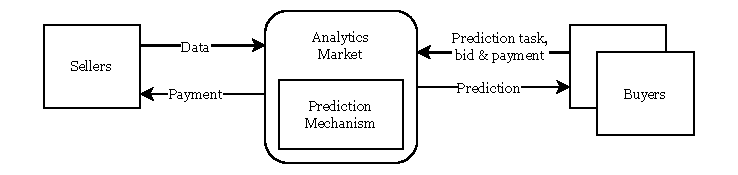
\includegraphics{Pictures/analytics_market.pdf}
  \caption{The setup of an analytics market. Sellers provide features and
  receive payment, and buyers provide a regression task and payment and receive
  a prediction.}
  \label{fig:analytics_market}
\end{figure}
\begin{figure}
  \centering
  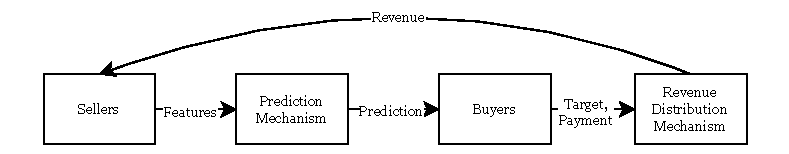
\includegraphics{Pictures/analytics_market_time_step.pdf}
  \caption{A single time step of the analytics market. Sellers provide
  features. These are passed through the machine learning model used by the
  market, which then forms a prediction. This prediction is supplied to buyers,
  who then give the true regression or classification target along with payment
  for the predictive improvement. Lastly, revenue is distributed between
  features by the market.}
  \label{fig:analytics_market_time_step}
\end{figure}

% An analytics market uses a regression or classification method to transform
% the features given from sellers to predictions for buyers. Buyers provide a
% prediction task, and sellers provide features for every clearing of the market.
% TODO These markets have been further developed to cover a wide range of
% situations.

Analytics markets are currently a research object and do not yet have a
real-world implementation. TODO:REF They were mathematically formalized in
TODO: REF AGARWAHL. Sellers receive payment based on a method from cooperative
game theory known as the Shapley value. The Shapley value payment distribution
is the unique distribution that fulfills a specific set of market properties
that in economics are known as the Shapley fairness properties.

The analytics market provides incentives for data sharing for the participants.
They are now paid based on how much their competitor benefits from receiving
their data, and everyone will be better off individually. The market
facilitates a cooperative environment by aligning incentives between the
participating parties. The situation is illustrated in figure
\ref{fig:wind_intro}, showing how adding a market can improve the outcome for
all participants.

\begin{figure}
  \centering
  \begin{subfigure}{.4\textwidth}
    \centering
    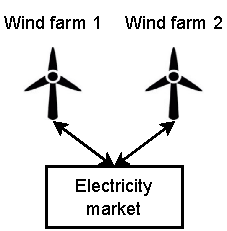
\includegraphics[width=.8\linewidth]{Pictures/wind_farm_double.pdf}
    \caption{Two wind farms in competition in the electricity market, each
    bidding individually but wanting each other's data.}
  \end{subfigure}%
  \hspace{1em}
\begin{subfigure}{.4\textwidth}
  \centering
  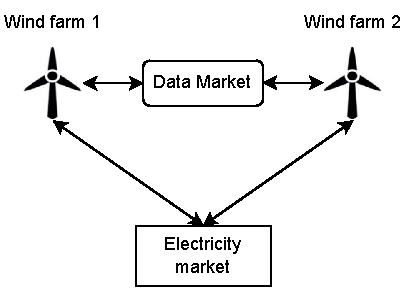
\includegraphics[width=.8\linewidth]{Pictures/wind_farms_two_with_market.pdf}
  \caption{Two wind farms exchanging data through the analytics market,
  incentivizing sharing and improving societal social welfare.}
\end{subfigure}%
  \caption{Motivating example showing how two wind farms will not voluntarily
  share data, but can be incentivized using an analytics market, improving
  social welfare for all of them.}
  \label{fig:wind_intro}
\end{figure}

Analytics market research up until this point has assumed that there is a fixed
number of agents in the market that will be present at all market clearings.
This is a strong assumption since agents are individuals or organizations that
naturally change their goals and status over time. For example, if a wind farm
is dismantled, it would no longer be able to provide production information to
a regression market.

Therefore, I relax the assumption of a fixed set of market participants, as I
now allow agents to leave the market or temporarily abstain from providing
features, as well as allowing new agents to join the market. In the figure
\ref{fig:wind_missing}, we see how a market participant can be missing at some
point, and how we need a mechanism to deal with this.

%TODO : SHOULD BE SOMEWHERE ELSENon-stationarity in the data generating distribution has been addressed in
% earlier research in TODO:PINSON PAPER using what is known as Online Learning
% methods, where the regression method is updated continuously as new data is
% made available. However, there is no literature dealing with a varying set of
% market participants.
\begin{figure}
  \centering
  \begin{subfigure}{.4\textwidth}
    \centering
    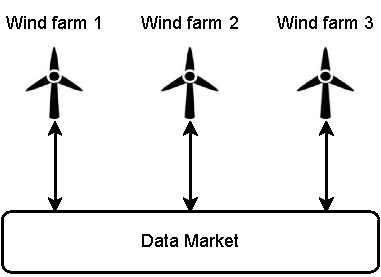
\includegraphics[width=.8\linewidth]{Pictures/data_market_3_wind_farms.pdf}
    \caption{At some time step in the market, all three of the shown wind farms
    are present in the market.}
  \end{subfigure}%
  \hspace{1em}
\begin{subfigure}{.4\textwidth}
  \centering
  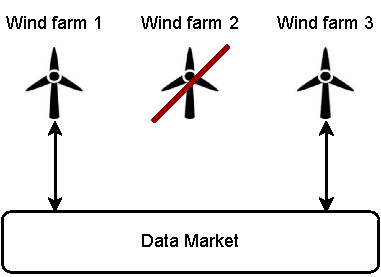
\includegraphics[width=.8\linewidth]{Pictures/data_market_3_wind_farms_missing.pdf}
  \caption{At another time, one wind farm is missing from the market, due to
  unforeseen events or maintenance or similar. The other two wind farms still
  want to participate.}
\end{subfigure}%
  \caption{A motivating example that shows how an analytics market can at one
  time have three present participants, but then one can go missing. This is a
  situation that current literature has not examined.}
  \label{fig:wind_missing}
\end{figure}

% TODO: REMOVE PROBABILISTIC
% The paper TODO:REF PINSON shows that in a two-price imbalance system, which is
% quite common in Europe, the optimal bid for an owner of a renewable energy
% generation resource is actually a certain quantile of their forecasted
% probability distribution. Therefore, it can be an improvement for market
% participants to use a probabilistic prediction method. For this reason, I also
% investigate online methods for probabilistic regression with a varying feature
% set.
%
\section{Literature Review}

TODO: REF PINS presents an analytics market in an online context. He shows that
a regression market can be constructed using any linear model optimizing a
convex loss function as the market model. However, he also assumes that the set
of features is constant, and so does not support adding or removing features.
In TODO: REF HAN, a regression market using the LASSO regressor is built, which
attempts to meet a need of both data buyers and data sellers. Sellers generally
want a minimum payoff before they are willing to disclose their feature, which
they can decide individually in the LASSO based market. Buyers also do not want
to pay for data that is barely informative, which is also avoided with this
regularized market. Thus, the market improves financial results for both buyers
and sellers.

A central issue within analytics markets is the problem of replication
robustness. The essence of the problem is that under the most common payment
policy, observational Shapley values, a participant can duplicate their own
data and sell it twice and thus increase their portion of the total revenue in
the market if other correlated features exist in the market. TODO: REF AGARWAHL
The paper TODO: REF REPLICATION-ROBUST investigates an alternative policy where
interventional shapley values are used, and shows that this payment policy is
robust to replication; however, it also includes higher financial risk to
market participants.

While online regression is one option for continuously updating a forecasting
mechanism over time, many participants instead use batch regression but retrain
their model every so often, often every day. TODO:REF This is equivalent to
using an online model to perform time-step-ahead predictions TODO:WRITE BETTER. One
alternative in this case for an online model that supports a varying number of
participants is a batch-learning model that supports the same. A framework for
this is presented in TODO:REF FCS PAPER that enables a batch learning approach
for arbitrary missing features using Fully Conditional Specification (FCS).

TODO: I SHOULD COMPARE TO FCS LATER

Online machine learning is the field of machine learning models that work not
on a batch of data in one go, but instead receiving data in a streaming
fashion. Online learning is usually based on an iterative updating of model
parameters one or a few time steps at a time TODO:REF. Online learning also
allows for the model to adapt to changes in the underlying data, i.e. a
non-stationary distribution. This can be done e.g. by exponential regretting
algorithms TODO:REF

Several state-of-the-art online learning models that support varying feature
spaces are presented in the survey article TODO:REF, where they name this
subfield Utilitarian Online Learning. The subfield is concerned with online
supervised learning models that are computationally efficient and can handle
arbitrarily varying feature spaces. The models presented are all classifiers,
and they create a taxonomy of three classes of utilitarian online learning
models that they classify them into. They do not present a regressor, which
will be needed for the market presented in this thesis.

There is then an open space in the literature both regarding a computationally
efficient regression mechanism for varying feature spaces, and regarding a
market built on one such mechanism, which would allow us to remove the
assumption that no participants enter or leave the data market.

\section{Contributions}

Motivated by this uninvestigated problem space, we would like to develop a
method for dealing with a varying number of participants in the market over
time. An analytics market requires a regression mechanism that can work with
the dynamics of its dataset, so we will need to investigate regression
mechanisms that work when the feature space varies over time. The regression
mechanism would be employed for multi horizon forecasting problems.

I will show that the newly introduced online regression mechanisms with
varying features fulfill the same properties for revenue distribution as seen
in previous research, covering Shapley fairness, truthfulness, and individual
rationality when using the traditional Shapley payment policy.

Additionally, I will examine methods for distributing revenue in markets with a
changing set of participants. I will show that some alternatives that one might
consider to the traditional Shapley value do not fulfill the above properties,
and I will show the consequences of using the Shapley value in varying feature
space. TODO: SHOW THE DON'T PAY MISSING OPTION.

TODO: Ref A Gal-Or 1985

TODO: EXPLAIN HOW TIME AHEAD FORECASTING IS EQUIVALENT TO BATCH LEARNING THAT DOES NOT RETRAIN.



